\documentclass[lang=cn,newtx,10pt,scheme=chinese]{../../elegantbook}

\title{数据结构百题狂练}
\subtitle{北街学长倾力之作}

\author{北街}
\date{2025/07/31}
\version{1.0}


\setcounter{tocdepth}{3}

\logo{../../figure/logo-blue.png}
\cover{../../figure/cover.jpg}

% 本文档命令
\usepackage{array}
\usepackage{longtable}
\usepackage{booktabs}
\newcommand{\ccr}[1]{\makecell{{\color{#1}\rule{1cm}{1cm}}}}

% 修改标题页的橙色带
\definecolor{customcolor}{RGB}{32,178,170}
\colorlet{coverlinecolor}{customcolor}
\usepackage{cprotect}

\addbibresource[location=local]{reference.bib} % 参考文献,不要删除
\usepackage{listings}         % 导入listings宏包
\usepackage{xcolor}           % 支持颜色
\usepackage{graphicx}        % 支持图形
% 配置C++代码样式
\lstset{
    language=C++,             % 语言设置为C++
    basicstyle=\ttfamily,      % 基本样式
    keywordstyle=\color{blue}, % 关键词颜色
    commentstyle=\color[rgb]{0,0.5,0},% 注释颜色  stringstyle=\color{red},   % 字符串颜色
    numbers=left,              % 显示行号
    numberstyle=\tiny,         % 行号样式
    stepnumber=1,              % 每行显示行号
    breaklines=true,           % 自动换行
    frame=lines                % 代码块边框样式
}

\usepackage{tikz}
\usetikzlibrary{chains, positioning, arrows.meta}
\begin{document}

\maketitle
\frontmatter

\tableofcontents

\mainmatter


\chapter{顺序表}



\begin{enumerate}
\def\labelenumi{\arabic{enumi}.}
\item
  
  从顺序表中删除具有最小值的元素(假设唯一),并由函数返回被删除的值,空出的位置有最后一个元素代替,若顺序表为空则显示错误信息并退出运行。
  
\end{enumerate}

\begin{table}[!htbp]
\centering
\begin{tabular}{|c|c|c|c|c|c|}
\hline
5 & 3 & 1 & 2 & 7 & 9 \\
\hline
\end{tabular}
\end{table}

\begin{enumerate}
\def\labelenumi{\arabic{enumi}.}
\setcounter{enumi}{1}
\vspace{5cm}
\item
  
  删除顺序表中值为x的元素(x可以不止一个),例如x=2
  
\end{enumerate}

\begin{table}[!htbp]
\centering
\begin{tabular}{c|c|c|c|c|c|c|}
\cline{2-7}
before delete: & 5 & 3 & 1 & 2 & 7 & 2 \\
\cline{2-7}
\end{tabular}
\end{table}

\begin{table}[!htbp]
\centering
\begin{tabular}{c|c|c|c|c|}
\cline{2-5}
after delete: & 5 & 3 & 1 & 7 \\
\cline{2-5}
\end{tabular}
\end{table}
\begin{enumerate}
\def\labelenumi{\arabic{enumi}.}
\setcounter{enumi}{2}
\vspace{5cm}
\item
  
  删除有序顺序表中重复的值,使表中所有的元素不同。
  
\end{enumerate}

\begin{table}[!htbp]
\centering
\begin{tabular}{c|c|c|c|c|c|c|}
\cline{2-7}
before delete: & 1 & 2 & 2 & 3 & 3 & 5 \\
\cline{2-7}
\end{tabular}
\end{table}

\begin{table}[!htbp]
\centering
\begin{tabular}{c|c|c|c|c|}
\cline{2-5}
after delete: & 1 & 2 & 3 & 5 \\
\cline{2-5}
\end{tabular}
\end{table}

\begin{enumerate}
\def\labelenumi{\arabic{enumi}.}
\setcounter{enumi}{3}
\vspace{5cm}
\item
  
  从有序顺序表中删除给定区间s-t之间的值(包含s和t),若给定区间不合理或顺序表为空,则显示错误信息并退出。
  
\end{enumerate}

\begin{table}[!htbp]
\centering
\begin{tabular}{c|c|c|c|c|c|c|}
\cline{2-7}
before delete: & 1 & 2 & 2 & 3 & 3 & 5 \\
\cline{2-7}
\end{tabular}
\end{table}

给定:s=1,t=3

\begin{table}[!htbp]
\centering
\begin{tabular}{c|c|}
\cline{2-2}
after delete: & 5 \\
\cline{2-2}
\end{tabular}
\end{table}
\begin{enumerate}
\def\labelenumi{\arabic{enumi}.}
\setcounter{enumi}{4}
\vspace{5cm}
\item
  
  假设表示集合的顺序表是一个有序顺序表,设计一个高效的算法实现集合的求差集运算,即C=A-B
  

  
\end{enumerate}

\begin{table}[!htbp]
\centering
\begin{tabular}{c|c|c|c|c|c|c|}
\cline{2-7}
A: & 1 & 2 & 2 & 3 & 3 & 4 \\
\cline{2-7}
\end{tabular}
\end{table}



\begin{table}[!htbp]
\centering
\begin{tabular}{c|c|c|c|c|c|c|}
\cline{2-7}
B: & 2 & 2 & 2 & 3 & 3 & 5 \\
\cline{2-7}
\end{tabular}
\end{table}

\begin{enumerate}
\def\labelenumi{\arabic{enumi}.}
\setcounter{enumi}{5}

\begin{table}[!htbp]
\centering
\begin{tabular}{c|c|c|}
\cline{2-3}
C: & 1 & 4 \\
\cline{2-3}
\end{tabular}
\end{table}
\vspace{5cm}
\item
  
  【2011统考真题】一个长度为L(L≥1)的升序序列S,处在第⌈L/2⌉个位置的数称为S的中位数。例如,若序列S1=(11,13,15,17,19
  ),则S1的中位数是15,两个序列的中位数是含它们所有元素的升序序列的中位数。例如,若S2=(2,4,6,8,20),则S1和S2的中位数是11。现在有两个等长升序序列A和B,试设计一个在时间和空间两方面都尽可能高效的算法,找出两个序列A和B的中位数。
  


\end{enumerate}

\begin{table}[!htbp]
\centering
\begin{tabular}{c|c|c|c|c|c|c|}
\cline{2-7}
A: & 1 & 2 & 4 & 6 & 7 & 8 \\
\cline{2-7}
\end{tabular}
\end{table}



\begin{table}[!htbp]
\centering
\begin{tabular}{c|c|c|c|c|c|c|}
\cline{2-7}
B: & 4 & 5 & 7 & 9 & 11 & 13 \\
\cline{2-7}
\end{tabular}
\end{table}

\begin{enumerate}
\def\labelenumi{\arabic{enumi}.}
\setcounter{enumi}{6}
\vspace{5cm}
\item
  
  将两个升序顺序表合并成一个新的顺序表,并由函数返回新的结果顺序表。
  


\end{enumerate}

\begin{table}[!htbp]
\centering
\begin{tabular}{c|c|c|c|c|c|c|}
\cline{2-7}
A: & 1 & 2 & 4 & 6 & 7 & 8 \\
\cline{2-7}
\end{tabular}
\end{table}



\begin{table}[!htbp]
\centering
\begin{tabular}{c|c|c|c|c|c|c|}
\cline{2-7}
B: & 4 & 5 & 7 & 9 & 11 & 13 \\
\cline{2-7}
\end{tabular}
\end{table}

\begin{table}[!htbp]
\centering
\begin{tabular}{c|c|c|c|c|c|c|c|c|c|c|}
\cline{2-11}
after merge: & 1 & 2 & 4 & 5 & 6 & 7 & 8 & 9 & 11 & 13 \\
\cline{2-11}
\end{tabular}
\end{table}

\begin{enumerate}
\def\labelenumi{\arabic{enumi}.}
\setcounter{enumi}{7}
\vspace{5cm}
\item
  
  实现一个空间复杂度为O(1)的顺序表逆置算法。
  
\end{enumerate}

\begin{table}[!htbp]
\centering
\begin{tabular}{c|c|c|c|c|c|c|}
\cline{2-7}
before reverse: & 1 & 2 & 4 & 6 & 7 & 8 \\
\cline{2-7}
\end{tabular}
\end{table}

\begin{table}[!htbp]
\centering
\begin{tabular}{c|c|c|c|c|c|c|}
\cline{2-7}
after reverse: & 8 & 7 & 6 & 4 & 2 & 1 \\
\cline{2-7}
\end{tabular}
\end{table}

\begin{enumerate}
\def\labelenumi{\arabic{enumi}.}
\setcounter{enumi}{8}
\vspace{5cm}
\item
  
  将arr中的存放的数据循环左移p个位置,即将arr中的(X0,X1,...,Xn-1变换为(Xp,Xp-1,...,Xn-1,X0,X1,...,Xp-1)),尽可能高效
  
\end{enumerate}

\begin{table}[!htbp]
\centering
\begin{tabular}{c|c|c|c|c|c|c|}
\cline{2-7}
p=3: & 1 & 2 & 4 & 6 & 7 & 8 \\
\cline{2-7}
\end{tabular}
\end{table}

\begin{table}[!htbp]
\centering
\begin{tabular}{c|c|c|c|c|c|c|}
\cline{2-7}
p=3: & 6 & 7 & 8 & 1 & 2 & 4 \\
\cline{2-7}
\end{tabular}
\end{table}

\chapter{单链表}

\begin{enumerate}
\def\labelenumi{\arabic{enumi}.}
\item
  
  单链表的基本操作:创建一个空链表、创建有值的单链表、输出单链表、输出单链表的长度、判断单链表是否为空、输出单链表的第k个元素、输出指定元素的位置、在第k个元素位置上插入f元素、删除单链表的第k个元素、释放单链表。
  
\vspace{5cm}
\item
  
  删除单链表中的唯一的最小值。

  \vspace{1cm}  

  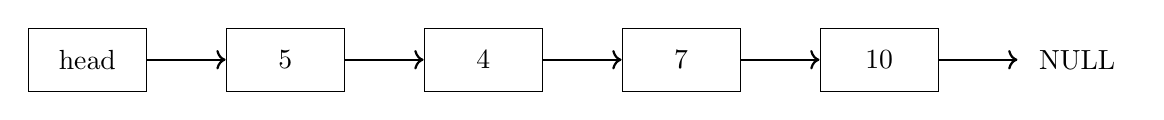
\begin{tikzpicture}[
    node distance = 1cm,
    start chain = going right,
    every node/.style = {
        draw, rectangle, minimum width=1.5cm, minimum height=0.8cm,
        on chain, join=by {->, thick}
    }
]
    % 定义链表节点
    \node {head};  % 节点1
    \node {5};  % 节点1
    \node {4};  % 节点2
    \node {7};  % 节点3
    \node {10};  % 最后一个节点N
    \node[draw=none, join=by {}] {NULL};  % NULL 指针(不画边框)
\end{tikzpicture}

\vspace{1cm}
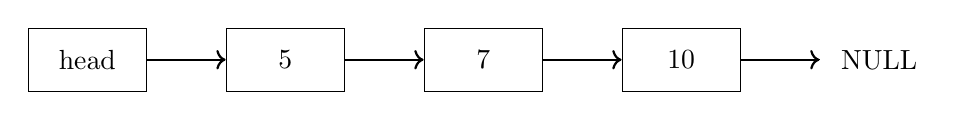
\begin{tikzpicture}[
  node distance = 1cm,
  start chain = going right,
  every node/.style = {
      draw, rectangle, minimum width=1.5cm, minimum height=0.8cm,
      on chain, join=by {->, thick}
  }
]
  % 定义链表节点
  \node {head};  % 节点1
  \node {5};  % 节点1
  \node {7};  % 节点2
  \node {10};  % 最后一个节点N
  \node[draw=none, join=by {}] {NULL};  % NULL 指针(不画边框)
\end{tikzpicture}

  
\vspace{5cm}
\item
  
  删除单链表中序号为奇数的结点(序号从首元结点开始)。

  \vspace{1cm}
  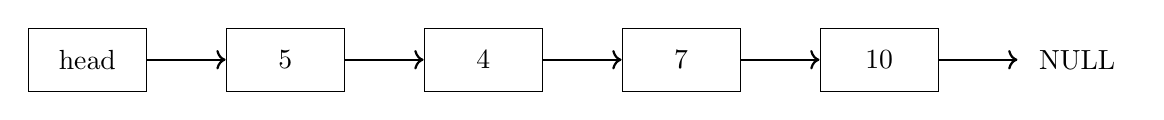
\begin{tikzpicture}[
    node distance = 1cm,
    start chain = going right,
    every node/.style = {
        draw, rectangle, minimum width=1.5cm, minimum height=0.8cm,
        on chain, join=by {->, thick}
    }
  ]
    \node {head};  % 节点1
    \node {5};  % 节点1
    \node {4};  % 节点2
    \node {7};  % 节点3
    \node {10};  % 最后一个节点N
    \node[draw=none, join=by {}] {NULL};  % NULL 指针(不画边框)
\end{tikzpicture}

\vspace{1cm}

  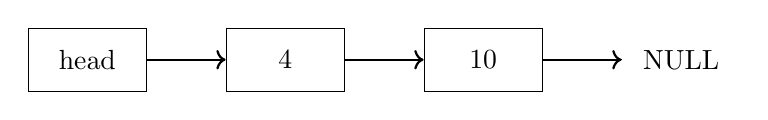
\begin{tikzpicture}[
    node distance = 1cm,
    start chain = going right,
    every node/.style = {
        draw, rectangle, minimum width=1.5cm, minimum height=0.8cm,
        on chain, join=by {->, thick}
    }
  ]
    \node {head};  % 节点1
    \node {4};  % 节点2
    \node {10};  % 最后一个节点N
    \node[draw=none, join=by {}] {NULL};  % NULL 指针(不画边框)
\end{tikzpicture}

  
  
  
\vspace{5cm}
\item
  
  设一个带头结点的单链表所有元素的数据值\textbf{无序},试编写函数删除表中介于给定的两个值(作为函数参数给出)之间的元素。例如,删除表中介于2和7之间的元素,如下图所示:

  \vspace{1cm}

  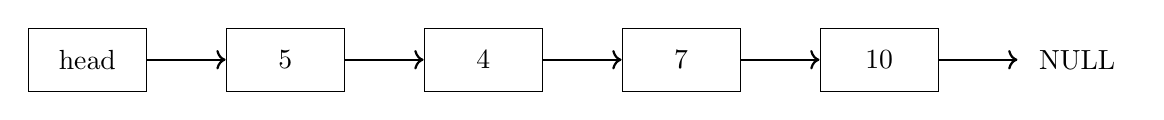
\begin{tikzpicture}[
    node distance = 1cm,
    start chain = going right,
    every node/.style = {
        draw, rectangle, minimum width=1.5cm, minimum height=0.8cm,
        on chain, join=by {->, thick}
    }
  ]
    \node {head};  % 节点1
    \node {5};  % 节点1
    \node {4};  % 节点2
    \node {7};  % 节点3
    \node {10};  % 最后一个节点N
    \node[draw=none, join=by {}] {NULL};  % NULL 指针(不画边框)
\end{tikzpicture}

\vspace{1cm}

  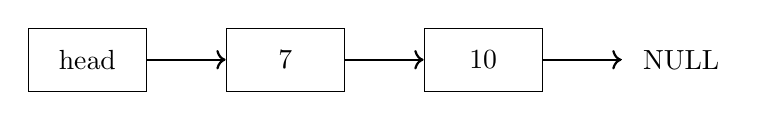
\begin{tikzpicture}[
    node distance = 1cm,
    start chain = going right,
    every node/.style = {
        draw, rectangle, minimum width=1.5cm, minimum height=0.8cm,
        on chain, join=by {->, thick}
    }
  ]
    \node {head};  % 节点1
    \node {7};  % 节点3
    \node {10};  % 最后一个节点N
    \node[draw=none, join=by {}] {NULL};  % NULL 指针(不画边框)
\end{tikzpicture}

\vspace{5cm}
\item
  
  设一个带头结点的单链表所有元素的数据值\textbf{递增有序},试编写函数删除表中介于给定的两个值(作为函数参数给出)之间的元素。例如,删除表中介于2和7之间的元素,如下图所示:

  \vspace{1cm}

  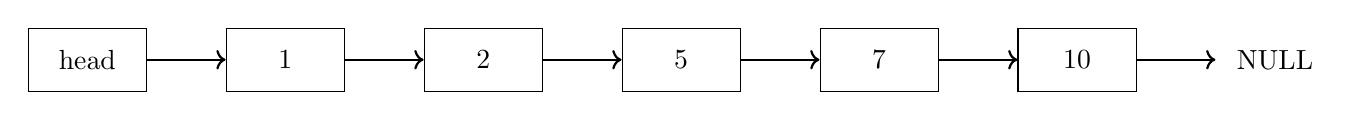
\begin{tikzpicture}[
    node distance = 1cm,
    start chain = going right,
    every node/.style = {
        draw, rectangle, minimum width=1.5cm, minimum height=0.8cm,
        on chain, join=by {->, thick}
    }
  ]
    \node {head};  % 节点1
    \node {1};  % 节点3
    \node {2};  % 节点3
    \node {5};  % 节点3
    \node {7};  % 节点3
    \node {10};  % 最后一个节点N
    \node[draw=none, join=by {}] {NULL};  % NULL 指针(不画边框)
\end{tikzpicture}

\vspace{1cm}

  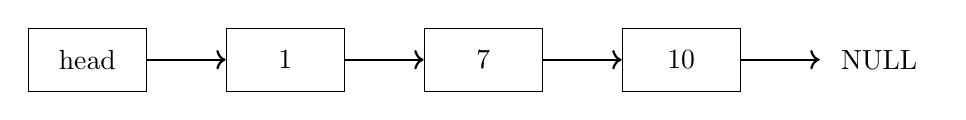
\begin{tikzpicture}[
    node distance = 1cm,
    start chain = going right,
    every node/.style = {
        draw, rectangle, minimum width=1.5cm, minimum height=0.8cm,
        on chain, join=by {->, thick}
    }
  ]
    \node {head};  % 节点1
    \node {1};  % 节点3
    \node {7};  % 节点3
    \node {10};  % 最后一个节点N
    \node[draw=none, join=by {}] {NULL};  % NULL 指针(不画边框)
\end{tikzpicture}

\vspace{5cm}
\item
  
  在一个\textbf{递增有序}的线性表中,有数值相同的元素存在,若存储方式为单链表,设计算法去掉数值相同的元素,使表中不再有重复的元素。

  
  
\vspace{5cm}
\item
  
  用单链表保存m个整数,结点的结构为{[}data{]}{[}next{]},且\textbar data\textbar\textless=n。现要求设计一个时间复杂度尽可能高效算法,对于链表中绝对值相等的结点,仅保留第一次出现的结点而删除其余绝对值相等的结点。
  
\vspace{5cm}
\item
  
  在带头结点的单链表L中,删除所有值为X的结点,并释放其空间,假设值为X的结点不唯一
  
\vspace{5cm}
\item
  
  设计一个递归算法,删除一个\textbf{不带头结点}的单链表中所有值为x的结点
  
\vspace{5cm}
\item
  
  将一个带头结点单链表A分解成两个带头结点的单链表A和B,使得A中含有原表中序号为奇数的元素,B中含有原表中序号为偶数的元素,且保持其相对位置不变。
  
\vspace{5cm}
\item
  
  设A、B是两个单链表(带头结点),其中元素\textbf{递增有序},设计一个算法从A、B中的公共元素产生单链表C,要求不破坏A、B结点
  
\vspace{5cm}
\item
  
  存在这样一种情况,如果两个单词有相同的后缀,那我们可以将后缀作为公共部分存储,比如being和loading,其中ing就可以作为公共部分,现在存在两个链表,含有公共部分,设计一个高效算法找到其公共后缀真实位置。
  
\vspace{5cm}
\item
  
  设计一个算法找到单链表中最后一个最小值。
  
\vspace{5cm}
\item
  
  求单链表中的中间位置结点元素,结点为偶数则向上取整。
  
\vspace{5cm}
\item
  
  有一个带头结点的单链表,设计一个函数找到指定的倒数第k个结点,输出结点值,并返回1,否则返回0,前提不能改变链表,尽可能高效。
  
\vspace{5cm}
\item
  
  设计算法在单链表中的第一个最大值前面插入值为x的结点。
  
\vspace{5cm}
\item
  
  判断单链表是否是升序(带头结点)。
  
\vspace{5cm}
\item
  
  设计一个算法判断一个单链表是否有环。
  
\vspace{5cm}
\item
  
  存在两个单链表序列A、B,设计函数判断B是否为A的子序列。
  
\vspace{5cm}
\item
  
  假设有两个按元素值\textbf{递增}次序排列的线性表,均以单链表形式存储。请编写算法将这两个单链表归并为一个按元素递减的单链表,并要求利用原来两个单链表的结点存放归并后的单链表。
  
\vspace{5cm}
\item
  
  将单链表里的所有零元素移动到非零元素前面。
  
\vspace{5cm}
\item
  
  按\textbf{递增次序}输出单链表各结点的数据元素,并释放结点所占的存储空间。
  
\vspace{5cm}
\item
  
  设计一个算法就地逆置单链表。所谓就地指的是空间复杂度为O(1)。
  
\vspace{5cm}
\item
  
  有一带头结点的单链表,设计一算法从尾到头的输出每个结点的值。
  
\vspace{5cm}
\item
  
  有一个带头结点的单链表L,设计一个算法使其递增有序。
  

\end{enumerate}

\chapter{循环单链表、非循环双链表、循环双链表}
\begin{enumerate}
\def\labelenumi{\arabic{enumi}.}
\item
  
  创建循环单链表。
  
\vspace{5cm}
\item
  
  设有一个带头结点的循环单链表,其结点均为正值,设计一个算法,反复找出单链表中最小值输出并删除后释放,直到单链表为空,最后释放头结点。
  
\vspace{5cm}
\item
  
  已知带头结点的循环单链表L中至少有两个结点,每个结点的两个域为data和next,其中data的类型为整型。设计算法判断该链表中的每个值是否小于其后续两个结点之和。
  
\vspace{5cm}
\item
  
  有两个循环单链表,链表头指针分别为h1和h2,编写一个函数将链表h2连接到h1之后,要求连接后的链表仍保持循环链表形式。
  
\vspace{5cm}
\item
  
  创建双向链表。
  
\vspace{5cm}
\item
  
  设计算法在带头结点循环双链表删除data域为x 的结点。
  
\vspace{5cm}
\item
  
  有一个非空双向链表L,设计算法在第k个结点之后插入一个值为x的结点。
  
\vspace{5cm}
\item
  
  设头指针为L的带有表头结点的非循环双向链表,其每个结点中除有pred(前驱指针)、data(数据)和next(后继指针)域外,还有一个访问频度域freq。在链表被启用前,其值均初始化为零。每当在链表中进行一次Locate(L,x)运算时,令元素值为×的结点中freq域的值增1,并使此链表中结点保持按访问频度非增(递减)的顺序排列,同时最近访问的结点排在频度相同的结点前面,以便使频繁访问的结点总是靠近表头。试编写符合上述要求的Locate
  (L,x)运算的算法,该运算为函数过程,返回找到结点的地址,类型为指针型。
  
\vspace{5cm}
\item
  
  非循环带头结点双链表中,将p所指结点与其后继结点交换(p非尾结点)。
  
\vspace{5cm}
\item
  
  设计一个算法判断带头结点的循环双链表是否对称。
  
\vspace{5cm}
\item
  
  设计算法就地逆置双链表。就地是指空间复杂度为O(1)。
  
\vspace{5cm}
\item
  
  带头结点双链表,设计算法使其元素递增有序。
  
\end{enumerate}

  \chapter{栈和队列}

\begin{enumerate}
\def\labelenumii{\arabic{enumii}.}
\item
    顺序栈、链栈的创建及其基本操作。
  \vspace{5cm}
\item
    链队、循环队列的创建及其基本操作。
  \vspace{5cm}
\item
    利用一个栈实现以下递归函数的非递归计算。

    \includegraphics[width=3.50833in,height=0.91806in]{./images/image1.png}
  \vspace{5cm}
\item
    设单链表的表头指针为h,结点结构由data和next两个域构成,其中data域为字符型。试设计算法判断该链表的全部n个字符是否是中心对称,例如xyx,xyyx都是中心对称。
  \vspace{5cm}
\item
    某汽车轮渡口,过江渡船每次能载10辆车过江。过江车辆分为客车类和货车类,上渡船有如下规定:同类车先到先上船;客车先于货车上船,且每上4辆客车,才允许放上Ⅰ辆货车;若等待客车不足4辆,则以货车代替;若无货车等待,允许客车都上船。试设计一个算法模拟渡口管理。
  \vspace{5cm}
\item
    假设一个算法表达式包含圆括号、方括号、和花括号3种类型的括号,编写一个算法来判断表达式里的括号是否配对,以字符`\textbackslash0'作为算术表达式的结束符。
  \vspace{5cm}
\item
    有一个队列和一个栈,设计一个算法是队列中的元素逆置。
  \vspace{5cm}
\item
    设有两个栈s1、s2都采用顺序栈方式,并共享一个存储区,大小为max,为了尽量利用空间,减少溢出的可能,可采用栈顶相向、迎面增长的存储方式,试设计s1、s2有关入栈和出栈的算法。
  \vspace{5cm}
\item
    若希望循环队列中的元素都能得到利用,则需设置一个标志域tag,并以tag
    的值为0或1来区分队头指针front和队尾指针rear相同时的队列状态是``空''还是``满''。试编写此结构相应的入队和出队算法。
  \vspace{5cm}
\item
    按下图所示铁道进行车厢调度(注意,两侧铁道均为单向行驶道,火车调度站有一个用于调度的``栈道''),火车调度站的入口处有n节硬座和软座车厢(分别用H和S表示)等待调度,试编写算法,输出对这n节车厢进行调度的操作(即入栈或出栈操作)序列,以使所有的软座车厢都被调整到硬座车厢之前。

    \includegraphics[width=4.375in,height=1.88958in]{./images/image2.png}

  \end{enumerate}
  \chapter{树、二叉树}

\begin{enumerate}
\def\labelenumi{\arabic{enumi}.}
\item
  已知一课二叉树按顺序存储结构进行存储,设计一个算法,求编号分别为i和j的两个结点的最近的公共祖先结点的值。
\vspace{5cm}
\item
  二叉树的创建及其基本操作:先序递归、中序递归、后序递归。
\vspace{5cm}
\item
  利用递归遍历的简单应用:统计结点个数、输出所有叶子结点、求结点值为x的所在层次、求第k层结点个数、求指定值为x的结点的双亲结点p、求二叉树中的最大结点值。
\vspace{5cm}
\item
  试写出先序遍历的非递归算法。
\vspace{5cm}
\item
  试写出中序遍历的非递归算法。
\vspace{5cm}
\item
  试写出后序遍历的非递归算法。
\vspace{5cm}
\item
  试写出层次遍历的算法。
\vspace{5cm}
\item
  假设二叉树是用二叉链表存储,试设计一个算法,求先序遍历中第k(1\textless=k\textless=二叉树的结点个数)个结点的值。
\vspace{5cm}
\item
  求二叉树中距离根结点最近的叶子结点。
\vspace{5cm}
\item
  假设二叉树采取二叉链表存储结构存储,试设计一个算法,计算一颗给定的二叉树所有的双分支结点个数。
\vspace{5cm}
\item
  设计一个算法复制一颗二叉树。
\vspace{5cm}
\item
  设计一个算法将二叉树的叶结点按从左到右的顺序连成一个单链表,表头指针为head。二叉树按二叉链表方式存储,连接时用叶结点的右指针来存放单链表指针。
\vspace{5cm}
\item
  设一个二叉树各结点的值互不相同,其先序遍历序列和中序遍历序列分别存于两个一维数组A、B中,试编写算法建立该二叉树的二叉链表。
\vspace{5cm}
\item
  一颗二叉树以二叉链表的形式存储,编写一个算法判断其是否是一个完全二叉树。
\vspace{5cm}
\item
  采用递归的方式求二叉树的高度。
\vspace{5cm}
\item
  假设二叉树采用二叉链表存储结构,设计一个非递归算法求二叉树的高度。
\vspace{5cm}
\item
  已知二叉树以二叉链表存储,编写算法完成:对于树中每一个元素值为x的结点,删除以它为根的子树,并释放相应的空间。
\vspace{5cm}
\item
  请设计一个算法,将给定的表达式树,转换成等价的中缀表达式并输出。
\vspace{5cm}
\item
  假设二叉树采用二叉链表存储结构,设计一个算法,求非空二叉树的宽度(即具有结点数最多的那一层的结点个数)。
\vspace{5cm}
\item
  假设二叉树采取二叉链表存储结构存储,试编写算法打印值为x的结点的所有祖先,假设x的值不多于一个。
\vspace{5cm}
\item
  设有一颗满二叉树(所有结点值均不同),已知其先序序列为pre,设计一个算法求其后序序列post。
\vspace{5cm}
\item
  p、q分别为指向该二叉树中任意两个结点的指针,试编写算法ancestor(root,p,q,r),找到p、q的最近公共祖先结点r。
\vspace{5cm}
\item
  编写算法打印从根结点到所有叶子结点的路径。
\vspace{5cm}
\item
  设计算法,输出二叉树中第一条最长的路径长度,并输出此路径上各结点的值。
\vspace{5cm}
\item
  试编写一个算法将一颗二叉树的所有结点的左右子树进行交换。
\vspace{5cm}
\item
  二叉树的带权路径长度(WPL)是二叉树中所有叶结点的带权路径长度之和。给定一颗二叉树T,采用二叉链表存储,结点结构为left
  weight right试设计求T的WPL的算法。
\vspace{5cm}
\item
  编写一个算法判断给定的二叉树是否是二叉排序树。
\vspace{5cm}
\item
  设计一个算法,求出指定结点在给定二叉排序树中的层次。
\vspace{5cm}
\item
  利用二叉树遍历的思想编写一个判断二叉树是否是二叉平衡树的算法。
\vspace{5cm}
\item
  编写一个递归算法,在一棵有n个结点的、随机建立起来的二叉排序树上查找第k小的元素,并返回指向该结点的指针,要求算法的平均时间复杂度为O(logn)。二叉排序树的每个结点中除了data、lchild、rchild等数据成员外,增加一个count成员,保存以该结点为根的子树的结点个数。
\vspace{5cm}
\item
  编程求以孩子兄弟表示法存储的森林的叶子结点数。
\vspace{5cm}
\item
  以孩子兄弟链表为存储结构,请设计递归算法求树的高度。
\vspace{5cm}
\item
  从所给的树的层次遍历及其结点度数信息,构造孩子兄弟链表。
\vspace{5cm}
\item
  将二叉树先序线索化、中序线索化、后序线索化。
\vspace{5cm}
\item
  写出在中序线索二叉树里查找指定结点在后序的前驱结点的算法。
\vspace{5cm}
\item
  哈夫曼树及哈夫曼编码实现。

\end{enumerate}
\chapter{图}

\begin{enumerate}
\def\labelenumi{\arabic{enumi}.}
\item
  
  以邻接矩阵方式创建一幅图。
  
\vspace{5cm}
\item
  
  以邻接表方式创建一幅图。
  
\vspace{5cm}
\item
  
  写出从图的邻接表表示转换成邻接矩阵表示的算法。
  
\vspace{5cm}
\item
  
  广度优先遍历(邻接矩阵与邻接表)。
  
\vspace{5cm}
\item
  
  深度优先遍历(邻接矩阵与邻接表)。
  
\vspace{5cm}
\item
  
  写出深度优先遍历的非递归算法(图用邻接表给出)。
  
\vspace{5cm}
\item
  
  最小生成树之prime算法。
  
\vspace{5cm}
\item
  
  最小生成树之kruskal算法。
  
\vspace{5cm}
\item
  
  利用广度优先遍历求解无权图单源最短路径。
  
\vspace{5cm}
\item
  
  最短路径之dijkstra(邻接矩阵与邻接表)。
  
\vspace{5cm}
\item
  
  最短路径之floyd。
  
\vspace{5cm}
\item
  
  采用深度优先遍历判断是否存在由vi到vj的路径,图用邻接表存储。
  
\vspace{5cm}
\item
  
  采用广度优先遍历判断是否存在由vi到vj的路径,图用邻接表存储。
  
\vspace{5cm}
\item
  
  输出顶点vi到顶点vj的所有简单路径,图用邻接表存储。
  
\vspace{5cm}
\item
  
  输出顶点vi到顶点vj的长度为L的所有简单路径,图用邻接表存储。
  
\vspace{5cm}
\item
  
  输出经过顶点k的所有简单回路,图用邻接表存储。
  
\vspace{5cm}
\item
  
  【2021统考真题】已知无向连通图G由顶点集V和边集E组成,\textbar E\textbar\textgreater0,当G中度为奇数的顶点个数为不大于2的偶数时,G存在包含所有边且长度为\textbar E\textbar 的路径(称为EL路径)。设图G采用邻接矩阵存储,设计算法,判断是否存在EL路径。
  
\vspace{5cm}
\item
  
  在采用邻接表存储的图上统计连通分支数并输出每个连通分支的顶点。
  
\vspace{5cm}
\item
  
  邻接矩阵存储的图中设计算法求树的直径。(在一棵树中,每一条边都有权值,树中的两个点之间的距离,定义为连接两点的路径上边权之和,那么树上最远的两个点,他们之间的距离,就被称之为树的直径。)
  
\vspace{5cm}
\item
  
  邻接矩阵存储一个有向图,设计算法求该有向图的所有根。
  
\vspace{5cm}
\item
  
  设计一个算法,判断一个无向图是否是一棵树。
  
\vspace{5cm}
\item
  
  设计一个算法实现拓扑排序(图以邻接表方式给出)
  

\end{enumerate}

\chapter{查找与排序}

\begin{enumerate}
\def\labelenumi{\arabic{enumi}.}
\item
  
  折半查找(递归与非递归)。
  
\vspace{5cm}
\item
  
  直接插入算法实现。
  
\vspace{5cm}
\item
  
  希尔排序算法实现。
  
\vspace{5cm}
\item
  
  简单选择排序算法实现。
  
\vspace{5cm}
\item
  
  简单选择排序在单链表中使用。
  
\vspace{5cm}
\item
  
  冒泡排序算法实现。
  
\vspace{5cm}
\item
  
  双向冒泡算法实现。
  
\vspace{5cm}
\item
  
  快速排序算法实现。
  
\vspace{5cm}
\item
  
  有一数组存放着无序序列K1,K2,K3,...,Kn,现要求将Kn放在将元素排
  序后的正确位置上,试编写实现该功能的算法,要求比较关键字的次
  数不超过n。
  
\vspace{5cm}
\item
  
  堆排序算法实现。
  
\vspace{5cm}
\item
  
  编写算法判断一个序列是否是小根堆。
  
\vspace{5cm}
\item
  
  归并排序算法实现。
  
\vspace{5cm}
\item
  
  计数排序算法实现。
  
\vspace{5cm}
\item
  
  编写一个算法,使之能够在数组中找到第k小的元素。
  
\vspace{5cm}
\item
  
  设计一个算法:将顺序表中的奇数全部移到偶数前面(时间最少,空间最少)。
  
\vspace{5cm}
\item
  
  2016年408真题:集合A划分为A1、A2,个数分别为n1、n2,和分别为S1、S2,\textbar n1-n2\textbar 最小\textbar S1-S2\textbar 最大。
  
\end{enumerate}

\end{document}
